\documentclass[border=5pt]{standalone}
\usepackage{tikz}
\usetikzlibrary{calc}
\usepackage{amsmath}
\begin{document}
        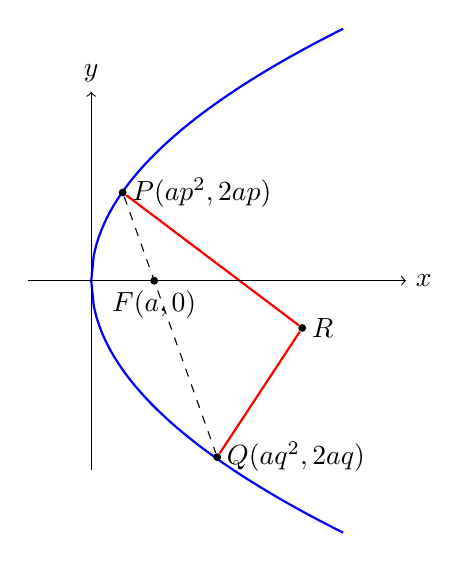
\begin{tikzpicture}[scale=0.8]
            % Draw parabola
            \draw[blue, thick, domain=0:4, samples=100] plot (\x, {sqrt(4*\x)});
            \draw[blue, thick, domain=0:4, samples=100] plot (\x, {-sqrt(4*\x)});

            % Draw points P and Q
            \node[circle, fill, inner sep=1pt] (P) at (0.5,1.4) {};
            \node[circle, fill, inner sep=1pt] (Q) at (2,-2.8) {};
            \node[right] at (P) {$P(ap^2,2ap)$};
            \node[right] at (Q) {$Q(aq^2,2aq)$};

            % Draw focus
            \node[circle, fill, inner sep=1pt] (F) at (1,0) {};
            \node[below] at (F) {$F(a,0)$};

            % Draw normals
            \node[circle, fill, inner sep=1pt] (R) at (3.35,-0.75) {};
            \node[right] at (R) {$R$};
            \draw[red, thick] (P) -- (R);
            \draw[red, thick] (Q) -- (R);

            % Draw chord PQ
            \draw[dashed] (P) -- (Q);

            % Draw axes
            \draw[->] (-1,0) -- (5,0) node[right] {$x$};
            \draw[->] (0,-3) -- (0,3) node[above] {$y$};
        \end{tikzpicture}
\end{document}
